\documentclass[]{book}

%These tell TeX which packages to use.
\usepackage{array,epsfig}
\usepackage{amsmath}
\newcommand{\Mod}[1]{\ (\text{mod}\ #1)}
\usepackage{amsfonts}
\usepackage{amssymb}
\usepackage{amsxtra}
\usepackage{amsthm}
\usepackage{mathrsfs}
\usepackage{algorithm}
\usepackage[noend]{algpseudocode}
\usepackage{color}
\usepackage{xcolor}
\usepackage{listings}
\usepackage{matlab-prettifier}
\usepackage{scrextend}
\usepackage{mathtools,calc}
\usepackage{caption}
\usepackage{subcaption}
\usepackage{float}
\usepackage{hyperref}
\hypersetup{
    colorlinks,
    linkcolor={red!50!black},
    citecolor={blue!50!black},
    urlcolor={blue!80!black}
}

%\usepackage{kbordermatrix}


\usepackage{color} %red, green, blue, yellow, cyan, magenta, black, white
\definecolor{mygreen}{RGB}{28,172,0} % color values Red, Green, Blue
\definecolor{mylilas}{RGB}{170,55,241}


%Here I define some theorem styles and shortcut commands for symbols I use often
\theoremstyle{definition}
\newtheorem{defn}{Definition}
\newtheorem{thm}{Theorem}
\newtheorem{cor}{Corollary}
\newtheorem*{rmk}{Remark}
\newtheorem{lem}{Lemma}
\newtheorem*{joke}{Joke}
\newtheorem{ex}{Example}
\newtheorem*{soln}{Solution}
\newtheorem{prop}{Proposition}

\newcommand{\lra}{\longrightarrow}
\newcommand{\ra}{\rightarrow}
\newcommand{\surj}{\twoheadrightarrow}
\newcommand{\graph}{\mathrm{graph}}
\newcommand{\bb}[1]{\mathbb{#1}}
\newcommand{\Z}{\bb{Z}}
\newcommand{\Q}{\bb{Q}}
\newcommand{\R}{\bb{R}}
\newcommand{\C}{\bb{C}}
\newcommand{\N}{\bb{N}}
\newcommand{\M}{\mathbf{M}}
\newcommand{\m}{\mathbf{m}}
\newcommand{\MM}{\mathscr{M}}
\newcommand{\HH}{\mathscr{H}}
\newcommand{\Om}{\Omega}
\newcommand{\Ho}{\in\HH(\Om)}
\newcommand{\bd}{\partial}
\newcommand{\del}{\partial}
\newcommand{\bardel}{\overline\partial}
\newcommand{\textdf}[1]{\textbf{\textsf{#1}}\index{#1}}
\newcommand{\img}{\mathrm{img}}
\newcommand{\ip}[2]{\left\langle{#1},{#2}\right\rangle}
\newcommand{\inter}[1]{\mathrm{int}{#1}}
\newcommand{\exter}[1]{\mathrm{ext}{#1}}
\newcommand{\cl}[1]{\mathrm{cl}{#1}}
\newcommand{\ds}{\displaystyle}
\newcommand{\vol}{\mathrm{vol}}
\newcommand{\cnt}{\mathrm{ct}}
\newcommand{\osc}{\mathrm{osc}}
\newcommand{\LL}{\mathbf{L}}
\newcommand{\UU}{\mathbf{U}}
\newcommand{\support}{\mathrm{support}}
\newcommand{\AND}{\;\wedge\;}
\newcommand{\OR}{\;\vee\;}
\newcommand{\Oset}{\varnothing}
\newcommand{\st}{\ni}
\newcommand{\wh}{\widehat}
\newcommand\independent{\protect\mathpalette{\protect\independenT}{\perp}}
   \def\independenT#1#2{\mathrel{\rlap{$#1#2$}\mkern2mu{#1#2}}}
\renewcommand{\theenumi}{\alph{enumi}}

%Pagination stuff.
\setlength{\topmargin}{-0.5 in}
\setlength{\oddsidemargin}{0in}
\setlength{\evensidemargin}{0in}
\setlength{\textheight}{9.5 in}
\setlength{\textwidth}{6.5in}
\urldef{\myurl}\url{http://download.springer.com/static/pdf/349/art%253A10.1186%252F1687-6180-2011-98.pdf?originUrl=http%3A%2F%2Fasp.eurasipjournals.springeropen.com%2Farticle%2F10.1186%2F1687-6180-2011-98&token2=exp=1482762525~acl=%2Fstatic%2Fpdf%2F349%2Fart%25253A10.1186%25252F1687-6180-2011-98.pdf*~hmac=d6d455ff5d3014b0387b6d1a327f3f02d5f8ca7e769a72bb6d903e4fff29a09f
}



\begin{document}
\hypersetup{
    colorlinks,
    linkcolor={red!50!black},
    citecolor={blue!50!black},
    urlcolor={blue!80!black}
}

\lstset{language=Matlab,%
    %basicstyle=\color{red},
    breaklines=true,%
    morekeywords={matlab2tikz},
    keywordstyle=\color{blue},%
    morekeywords=[2]{1}, keywordstyle=[2]{\color{black}},
    identifierstyle=\color{black},%
    stringstyle=\color{mylilas},
    commentstyle=\color{mygreen},%
    showstringspaces=false,%without this there will be a symbol in the places where there is a space
    numbers=left,%
    numberstyle={\tiny \color{black}},% size of the numbers
    numbersep=9pt, % this defines how far the numbers are from the text
    emph=[1]{for,end,break},emphstyle=[1]\color{red}, %some words to emphasise
    %emph=[2]{word1,word2}, emphstyle=[2]{style},
}

\begin{center}
{\Large Image Processing \hspace{0.5cm} Assignment 3 - Poisson Image Editing}\\
\textbf{Julien Siems (16119007)}\\ %You should put your name here
\end{center}

\vspace{0.2 cm}
\section*{Task 1}
\subsection*{Part a.)}
\subsubsection*{Problem statement}
The paper proposes a solution to seamless editing of image regions. 
It solves the following problems:
\begin{enumerate}
\item Seamless cloning of regions from a source image to a target image.
\item Seamless change of properties of an image inside a region.
\end{enumerate}


\subsubsection*{Key ideas}
One of the key ideas of this paper is the statement of the minimization problem. (Equation 3)
\begin{equation}
\min_f \iint_{\Omega} |\nabla f - \mathbf{v}|^2 \text{ with } f|_{\partial \Omega} = f^*|_{\partial \Omega}
\end{equation}

whose solution should satisfy the following Poisson equation.
\begin{equation}
\Delta f = \text{div} \mathbf{v} \text{ over } \Omega\text{, with } f|_{\partial \Omega} = f^*|_{\partial \Omega} \label{eq:poissondirich}
\end{equation}

The left part of \ref{eq:poissondirich} means that the second order variations of the domain $\Omega$ must agree with the divergence of the guidance vector field $\textbf{v}$. As described in the introduction of the paper, second order variations are more significant perceptually, than first order variations. Thus it is important for them to agree to make it look realistic.

The right part means that the function $f$ in domain $\Omega$ should agree on their boundary with the surrounding function $f^*$. This condition ensures a smooth transition between $\Omega$ and the surrounding domain.

Depending on the effect that is supposed to be achieved one can choose different
vector fields. This makes this technique very powerful.


\subsubsection*{Applications}
\begin{itemize}
\item Concealment: Can be achieved by picking as source image a region within the image that is similar to the target region. As guidance vector field we could choose either the laplacian of the source region or we could mix the gradients depending on which of them has a higher value. (Figure 2 in the paper)
\item Insertion: One picks a source region in one image and then inserts into a target image. This can be solved very similarly to the Concealment application. When objects with holes are inserted than using the mixed gradients technique which favours the higher gradíent of either the source or target image can result in a better output.
\item Selection editing:
\begin{itemize}
\item Texture flattening: Achieved using a sieve that leaves only the most prominent features(For example most important edges etc.). A possible guidance vector field is given in equation 15 in the paper.
\item Local illumination changes: Used for smooth dynamic range changes. Defined on the log domain to avoid arithmetic underflow. A possible guidance vector field is given in equation 16. To increase the dynamic range these changes are made in the log domain.
\item Local color changes: One possible application is turning everything but a region in an image monochrome. This is solved by setting $f^*$ to be the gray channel of itself. Then a region is picked in the original color $f^*$, which is inserted into the monochrome version using the approach described above for each color channel.
\item Seamless tiling: Acchieved by ensuring that the north south and east west borders agree.
\end{itemize}
\end{itemize}

\subsection*{Part b.)}
\subsubsection*{What I like in the paper}
\begin{itemize}
\item The changes look very complex and would also be time consuming to do manually. Still, the technique is fast.
\item I like the fact that the domains can have an arbitrary shape. 
\item The selections when cloning or when using selective editing don't have to be extremely accurate. They can be rather loose and still result in very good results.
\item Only the guidance vector field needs to be adjusted for different applications. It can be easy to illustrate and therefore to choose an appropriate vector field for the problem at hand.
\item The technique is very neat. It makes sense that the border values have to agree and that the domain is guided by the most prominent features of the source.
\item Technique can be applied to each color component independently.
\end{itemize}

\subsubsection*{What I don't like about the paper}
\begin{itemize}
\item Because the approach only takes into the account the laplacian of each color channel some information about the actual color of the source image is lost. This artefact can be seen in Figure 3. While the insertion of the bear is very seamless the bear suddenly has more of a bright blue color which doesn't match it's normal color. An improved version of the algorithm found was developed that takes the color into account.\footnote{Dizdaroğlu and İkibaş, An improved method for color image editing, EURASIP Journal on Advances in Signal Processing 2011, 2011:98}
\end{itemize}


\section*{Task 2}
\subsection*{Explanation and code}
Equation 2 from the paper assumes no prior knowledge of any guidance vector field inside the domain. The laplacian inside the region is supposed to be zero. However, the boundary values of the unknown function $f$ and the target function $f^*$ have to agree.

$A$ doesn't change in the LSE. $b$ becomes:
\begin{equation}
b_{p_i} = \sum_{q\in N_{p_i}\cap \partial \Omega} f_q^*
\end{equation}

Code listing:
\lstinputlisting[style=Matlab-editor, basicstyle=\footnotesize]{Code/ex2.m}


\subsection*{Results}
\begin{figure}[H]
\centering{}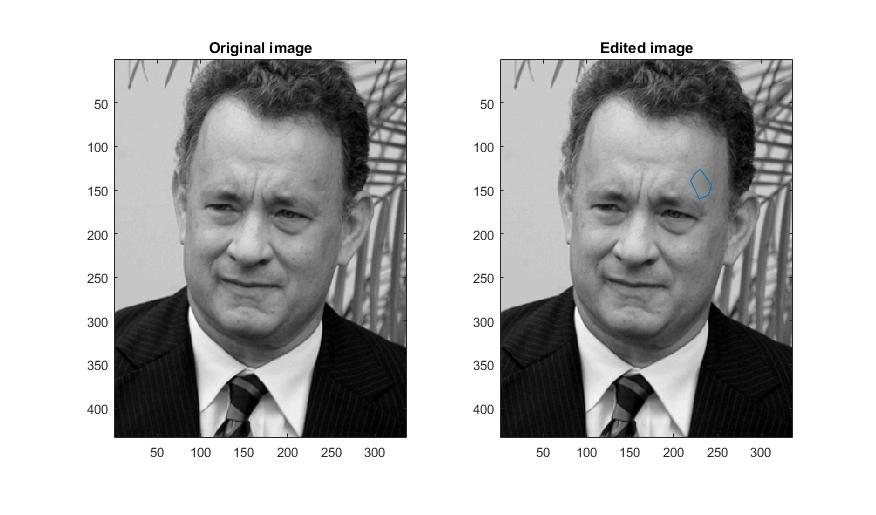
\includegraphics[width=13cm]{images/ex2_smooth.jpg}\caption{Interpolation of relatively small, smooth region.\label{ex2_smooth}}
\end{figure}
As can be seen in figure \ref{ex2_smooth} small, smooth regions can work very well without a guidance vector field. When zooming out however, it becomes apparent that the region is noticeably too smooth compared to the surrounding skin, since a zero laplacian is assumed inside the domain.

\begin{figure}[H]
\centering{}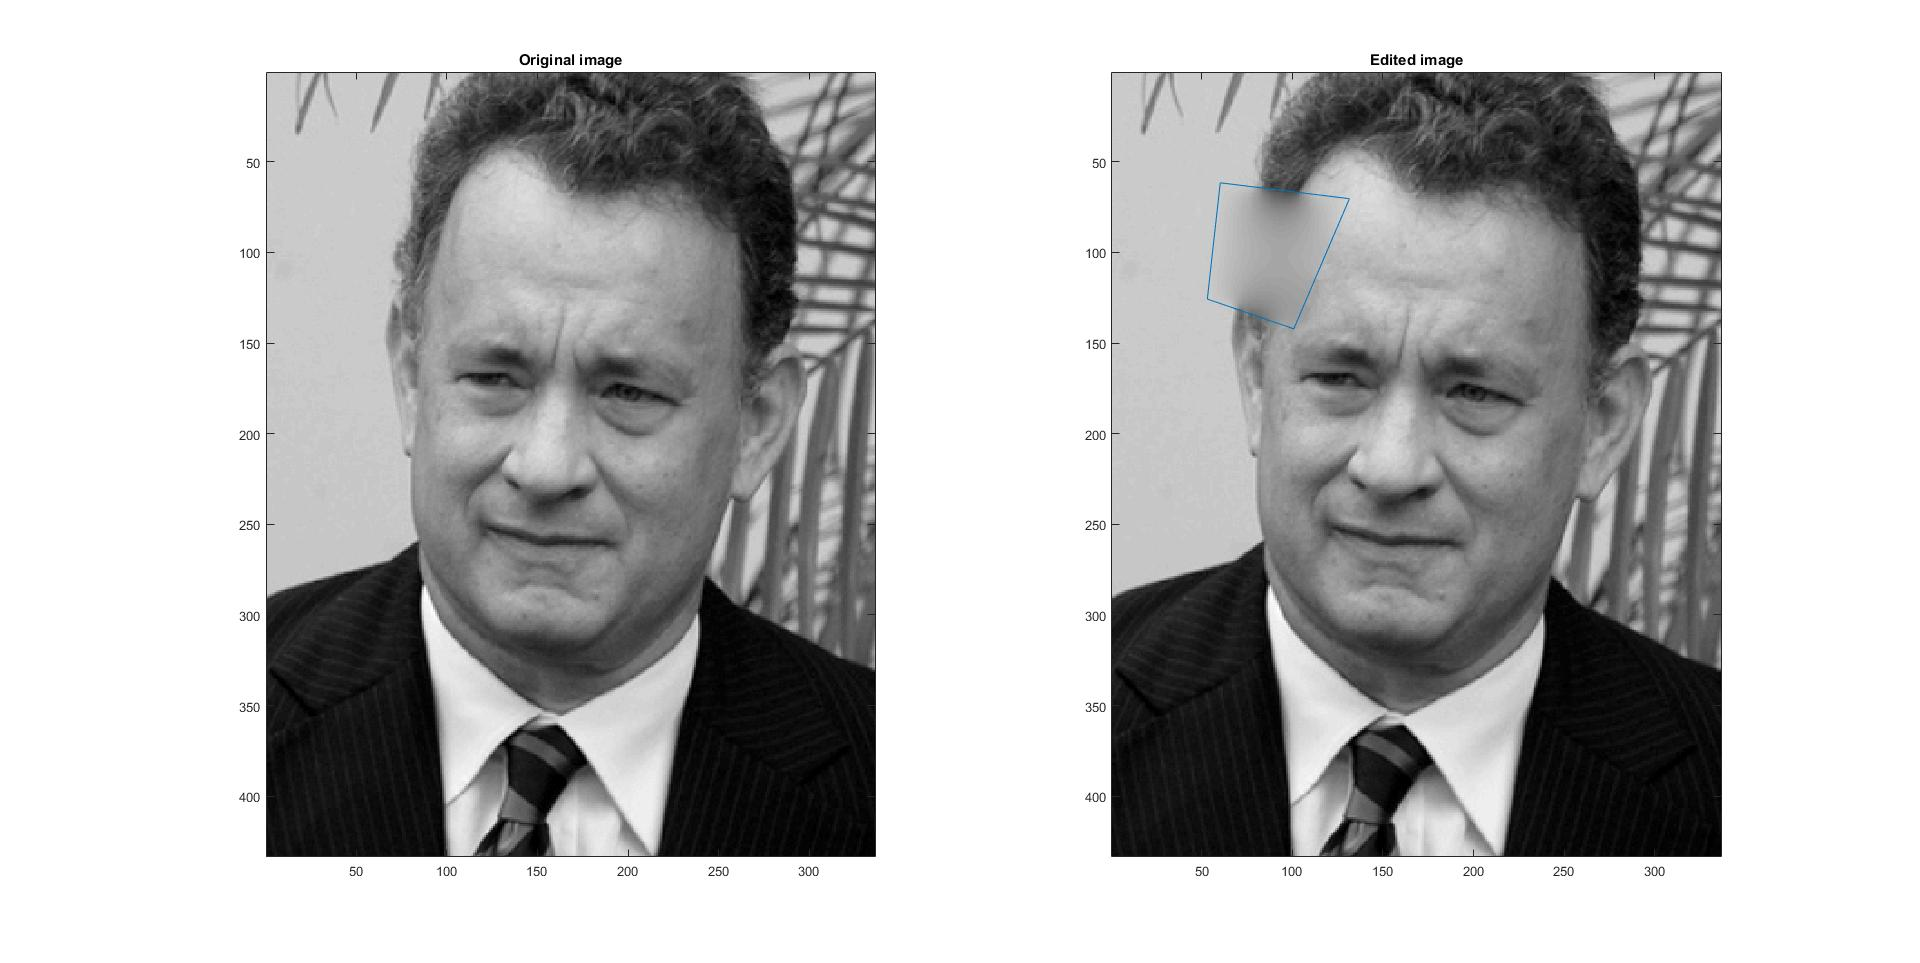
\includegraphics[width=13cm]{images/ex2_edges_big_region.jpg}\caption{Interpolation of bigger region with a lot of edges. \label{ex2_edges_big_region}}
\end{figure}
In figure \ref{ex2_edges_big_region} the true downside of not using a guidance vector field can be seen. Close to the boundary of the region the interpolation is still realistic but in the middle of the region it seems very blurred. This artifact was mentioned in the paper.

What can also be seen is that the bigger the region the less constrained the the interpolation becomes towards the middle of the region.

\section*{Task 3}

\end{document}